\chapter{Revisão bibliográfica}
\label{chapterRevisao}
\section{Transistores em circuitos de potência}
\label{sectionCap2transistores}
\subsection{Transistores de potência baseados em Silício}
Os transistores de potência baseados em silício, tiveram sua eficiência e o custo do gerenciamento de energia melhorado continuamente nas ultimas decadas. Inovações em estruturas do transistor acompanharam a crescente necessidade de equipamentos eletrônicos em nossas vidas diárias. No entanto, a taxa de melhoria diminuiu bastante, uma vez que, assintoticamente, se aproxima de seus limites teóricos. \cite{lidow_rooij_strydom_reusch_glaser_2020}

\subsection{Transistor baseados em Nitreto de Gálio (GaN)}
Dispositivos baseados em Nitreto de Gálio (GaN) apareceram pela primeira vez em cerca de 2004, como transistores de radiofrequência (RF) feitos pela Eudyna Corporation do Japão. Usando GaN em substratos de carbeto de silício (SiC), a Eudyna produziu transistores projetados para o mercado de RF, com sucesso \cite{Alex}. Porém, não só do ponto de vista de RF há vantagens em utilizar GaN, há vantagens também em eletrônica de potência. As caracteristicas dos dispositivos baseados em Nitreto de Gálio podem ser vistas na comparação da Tabela \ref{t_materiais}.

\begin{table}[!htb]
\centering
\caption{Comparação entre propriedades dos materiais \cite{lidow_rooij_strydom_reusch_glaser_2020}}
\begin{tabular}{lllll}
\hline
Parâmetro           &                & Si    & SiC   & GaN \\ \hline
Banda de Gap $E_g$& $(eV)$             & 1,12  & 3,39  & 3,26\\
Campo Elétrico crítico $E_{Crit}$ &$(MV/cm)$   & 0,23  & 3,3   & 2,2\\
Mobilidade dos elétrons $\mu_n$ &$(cm^2/V.s)$& 1400  & 1500  & 950\\
Permissividade $\varepsilon_r$ &     & 11,8  & 9     & 9,7\\
Condutividade térmica $\lambda$& $(W/cm.K)$     & 1,5   & 1,3   & 3,8\\ \hline
\end{tabular}
\label{t_materiais}
\end{table}

\subsubsection{Banda de Gap $(E_g)$}
A banda de Gap de um semicondutor está relacionado à força das ligações químicas entre os átomos na rede. Essas ligações mais fortes significam que é mais difícil para um elétron saltar de um nível para o próximo. Entre as muitas consequências estão correntes de fuga intrínsecas mais baixas e maiores temperaturas de operação para semicondutores de gap maior. Com base nos dados da Tabela \ref{t_materiais}, GaN e SiC têm banda de Gap maiores do que o silício. \cite{lidow_rooij_strydom_reusch_glaser_2020}

\subsubsection{Resistência quando ligado $(R_{DS_{(on)}})$}
\par A resistência teórica, em Ohms ($\Omega$), será dada pela equação \ref{RdsOn}. \cite{lidow_rooij_strydom_reusch_glaser_2020}
\begin{equation}
    R_{DS_{(on)}} = \frac{W_{drift}}{q.\mu_n .N_D}
    \label{RdsOn}
\end{equation}
\par A resistência, quando relacionada com o Campo Elétrico Crítico $(E_g)$ será dada por \ref{RdsOnEg}. \cite{lidow_rooij_strydom_reusch_glaser_2020}
\begin{equation}
    R_{DS_{(on)}} = \frac{4.V^2_{BR}}{\varepsilon_o .\varepsilon_r . E^3_{crit}}
    \label{RdsOnEg}
\end{equation}
\par A equação dada por \ref{RdsOnEg} está representada no gráfico da Figura \ref{FigRDSon}.
\begin{figure}[H]
\caption{Resistência $R_{DS_(on)}$ vs capacidade de bloquear tensão para dispositivos Si, SiC, and GaN \cite{lidow_rooij_strydom_reusch_glaser_2020}}
 \centering % para centralizarmos a figura
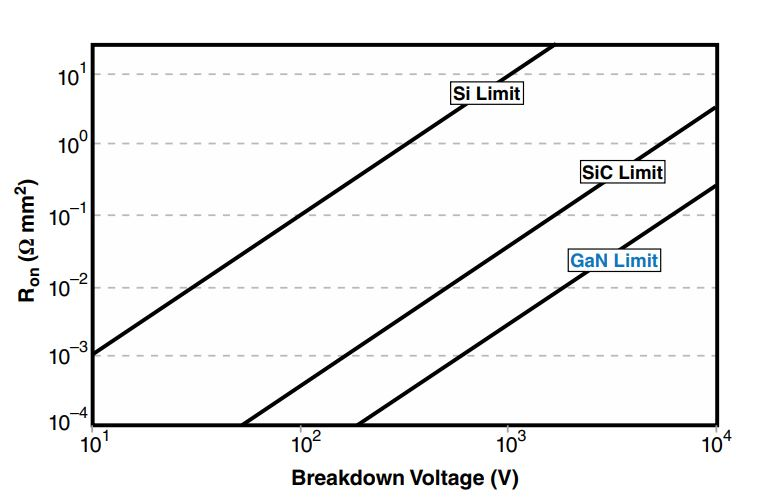
\includegraphics[width=10cm]{figuras/5.JPG} 
\label{FigRDSon}
\end{figure}
\noindent Junto com a baixa resistência $R_{DS_(on)}$, há o benefício de conseguir trabalhar em frequências mais altas que IGBTs com potências relativamente altas, como mostra a Figura \ref{FigComparison}. 
\begin{figure}[H]
\caption{Potência vs Frequência. \cite{Sameer}}
 \centering % para centralizarmos a figura
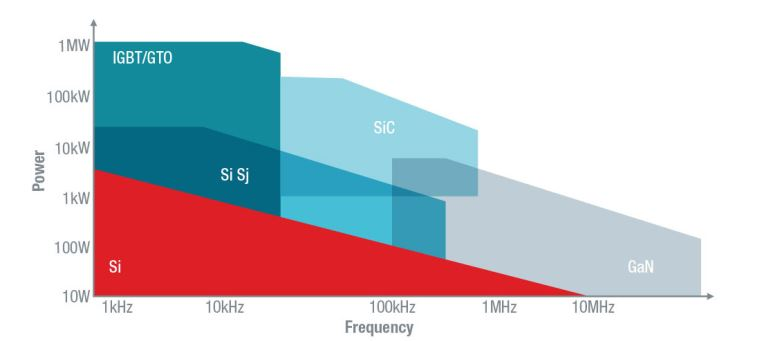
\includegraphics[width=14cm]{figuras/6.JPG} 
\label{FigComparison}
\end{figure}

%%%%%%%%%%%%%%%%%%%%%%%%%%%%%%%%%%%%%%%%%%%%%%%%%%%%%%%%%%%%%%%%%%%%%%%%%%%%%%%%%%%%%%%%%%%%%%%%%%%%%%%%%%%%%%%%
%%%%%%%%%%%%%%%%%%%%%%%%%%%%%%%%%%%%%%%%%%%%%%%%%%%%%%%%%%%%%%%%%%%%%%%%%%%%%%%%%%%%%%%%%%%%%%%%%%%%%%%%%%%%%%%%
%%%%%%%%%%%%%%%%%%%%%%%%%%%%%%%%%%%%%%%%%%%%%%%%%%%%%%%%%%%%%%%%%%%%%%%%%%%%%%%%%%%%%%%%%%%%%%%%%%%%%%%%%%%%%%%%
%%%%%%%%%%%%%%%%%%%%%%%%%%%%%%%%%%%%%%%%%%%%%%%%%%%%%%%%%%%%%%%%%%%%%%%%%%%%%%%%%%%%%%%%%%%%%%%%%%%%%%%%%%%%%%%%
%%%%%%%%%%%%%%%%%%%%%%%%%%%%%%%%%%%%%%%%%%%%%%%%%%%%%%%%%%%%%%%%%%%%%%%%%%%%%%%%%%%%%%%%%%%%%%%%%%%%%%%%%%%%%%%%
\section{Conversor abaixador de tensão (\textit{Buck})}
\label{sectionCap2Buck}
A aplicação dos transistores discutidos na seção \ref{sectionCap2transistores} se dará no conversor chaveado representado da figura \ref{figBuck}, um conversor abaixador de tensão, que aqui será chamado de conversor \textit{Buck}. 

\begin{figure}[H]
\caption{Conversor abaixador de tensão} 
\begin{center}
\begin{circuitikz}
%Coluna,Linha
%(0,0) botton left

\draw
    (6,4)   to [american voltage source, l_=$V_{in}$] (6,0)
    (6.6,4.2) node[]{$V_{in}$}
    %(6,0)   to [short,*-] (7,4)
    %(7,4)   to [short,*-] (8,4)
    (6,4)   to [short,-] (8,4)
    (8,4)   to [switch, l_=$T$] (10,4)
    %(6,4)   to [short,*-] (7,0)
    %(7,0)   to [short,*-] (14,0)
    (6,0)   to [short,-] (12,0)
    (12,0)   to [short,-] (15,0) 
    (8,0)   to [C,l_=$C_{in}$, *-*] (8,4)
    (10,0)  to [D,l_=$D$,*-*] (10,4)
    (10,4)  to [L,l_=$L$,i=$I_o$] (12,4) 
    (12,4)   to [short,-] (15,4) 
    (13,4)   to [C,l_=$C_{out}$,*-*] (13,0)
    (14,4.2) node[]{$V_{o}$}
    (15,4)  to [R,l_=$R_{o}$,-*] (15,0)
    node[ground]{};
\end{circuitikz}
\end{center}
\label{figBuck}
\end{figure}
\par O circuito da figura \ref{figBuck} é analisado dividindo-se o circuido em dois, presentes na figura \ref{figBuckChaveFechada}. Com a chave ($T$) aberta ou fechada:
\begin{itemize}
\item Chave fechada: tem-se o circuito com o diodo $D$ desligado (não conduzindo) e o indutor $L$ e capacitor $C$ sendo carregados (aumento de $I_o)$. 
\item Chave aberta: no instante que a chave $T$ é desligada (para de conduzir), o diodo $D$ conduz, dando continuidade à corrente do indutor $L$. A energia armazenada em $L$ é entregue ao capacitor $C$ e à carga. 
%Enquanto o valor instantâneo da corrente pelo indutor for maior do que a corrente da carga, a diferença carrega o capacitor. Quando a corrente for menor, o capacitor se descarrega, suprindo a diferença a fim de manter constante a corrente da carga (já que estamos supondo constante a tensão Vo). A tensão a ser suportada, tanto pelo transistor quanto pelo diodo é igual à tensão de entrada, E.
\end{itemize}
\par Caso o circuito opere no modo contínuo, a corrente pelo indutor não vai a zero durante a condução do diodo, caso contrario, opera no modo descontínuo. Neste trabalho, será utilizado no modo contínuo por possuir uma relação bem determinada entre a largura de pulso ($\delta$) e a tensão média de saída ($V_o$). \cite{pomilio}. 


\begin{figure}[H]
\caption{Conversor abaixador de tensão: Chave Fechada/Chave ligada} 

\begin{center}
\begin{circuitikz}
\draw[red,dashed,rounded corners=0.2cm,-latex]
           ($(7,1) + ( 0.175,-0.5  )$) 
        -- ($(7,4) + ( 0.175,-0.175)$) 
        -- ($(15,4)  - ( 0.175, 0.175)$)
        -- ($(15,0) + (-0.175, 0.175)$) 
        -- ($(8,0) + ( 0.175, 0.175)$)
    ;
    
\draw[red,dashed,rounded corners=0.2cm,-latex]
           ($(0,1) + ( 0.175,-0.5  )$) 
        -- ($(0,4) + ( 0.175,-0.175)$) 
        -- ($(5,4)  - ( 0.175, 0.175)$)
        -- ($(5,0) + (-0.175, 0.175)$) 
        -- ($(1,0) + ( 0.175, 0.175)$)
    ;
%Coluna,Linha
%(0,0) botton left
\draw
    (7,4)   to [american voltage source, l_=$V_{in}$,i=$I_T$] (7,0)
    (7.6,4.2) node[]{$V_{in}$}
    %(6,0)   to [short,*-] (7,4)
    %(7,4)   to [short,*-] (8,4)
    (7,4)   to [short,-] (10,4)
    %(6,4)   to [short,*-] (7,0)
    %(7,0)   to [short,*-] (14,0)
    (7,0)   to [short,-] (12,0)
    (12,0)   to [short,-] (15,0) 
    (9,0)   to [C,l_=$C_{in}$, *-*] (9,4)
    (10,4)  to [L,l_=$L$,i=$I_o$] (12,4) 
    (12,4)   to [short,-] (15,4) 
    (13,4)   to [C,l_=$C_{out}$,*-*] (13,0)
    (14,4.2) node[]{$V_{o}$}
    (15,4)  to [R,l_=$R_{o}$,-*] (15,0)
    node[ground]{};
    
   \draw
    (0,0)   to [short,-] (5,0)
    (0,0)  to [D,l_=$D$,i=$I_d$,-] (0,4)
    (0,4)  to [L,l_=$L$,i=$I_o$] (2,4) 
    (2,4)   to [short,-] (5,4) 
    (2.5,4)   to [C,l_=$C_{out}$,*-*] (2.5,0)
    (4,4.2) node[]{$V_{o}$}
    (5,4)  to [R,l_=$R_{o}$,-*] (5,0)
    node[ground]{};
\end{circuitikz}
\end{center}
\label{figBuckChaveFechada}
\end{figure}

\subsection{Equacionamento do conversor Buck}
Considerando operação em modo de condução contínua (MCC), quando o indutor $L$ nunca tem sua corrente indo a zero, tem-se o \textit{duty-cycle} ($\delta$) dado pela equação \ref{MCCduty} \cite{pomilio}.
\begin{equation}
    \frac{V_o}{V_{in}} = \delta
    \label{MCCduty}
\end{equation}
Conhecendo-se o periodo ($\tau$), a corrente $I_{o(min)}$ será dada pela \ref{BuckIo} \cite{pomilio}.
\begin{equation}
    I_{o(min)}=\frac{(V_{in}-V_o).\delta.\tau}{2.L}
    \label{BuckIo}
\end{equation}
E para se operar sempre no modo contínuo, o indutor $L$ mínimo deverá ser dado pela equação \ref{Lmin} \cite{pomilio}.
\begin{equation}
    L_{min}=\frac{V_{in}.(1-\delta).\delta.\tau}{2.I{o(min)}}
    \label{Lmin}
\end{equation}
O capacitor de saída $C_o$ será dimensionado pela equação \ref{Co} e a variação da tensão de saída $\Delta V_o$ pela equação \ref{DeltaVo} \cite{pomilio}.
\begin{equation}
    C_{o}=\frac{V_o.(1-\delta).\tau^2}{8.L.\Delta V_o}
    \label{Co}
\end{equation}
\begin{equation}
    \Delta V_{o}=\frac{\tau^2.V_{in}.\delta.(1-\delta).}{8.L.\Delta C_o}
    \label{DeltaVo}
\end{equation}
\section{Painel solar}
\par Um sistema solar fotovoltáico é um sistema que converte luz solar em eletricidade. Esse sistema se baseia em uma célula fotovoltaica que formarão paineis fotovoltáicos, após agrupadas. 
\par Ao ser iluminado, os terminais de saída do painel fotovoltaico fornecerão energia elétrica e o perfil de potência (curva $I-V$) é dado pela imagem \ref{FigPVprofile}.

\begin{figure}[H]
\caption{Curva I-V. Retirada de \cite{VillalvaRuppert}}
 \centering % para centralizarmos a figura
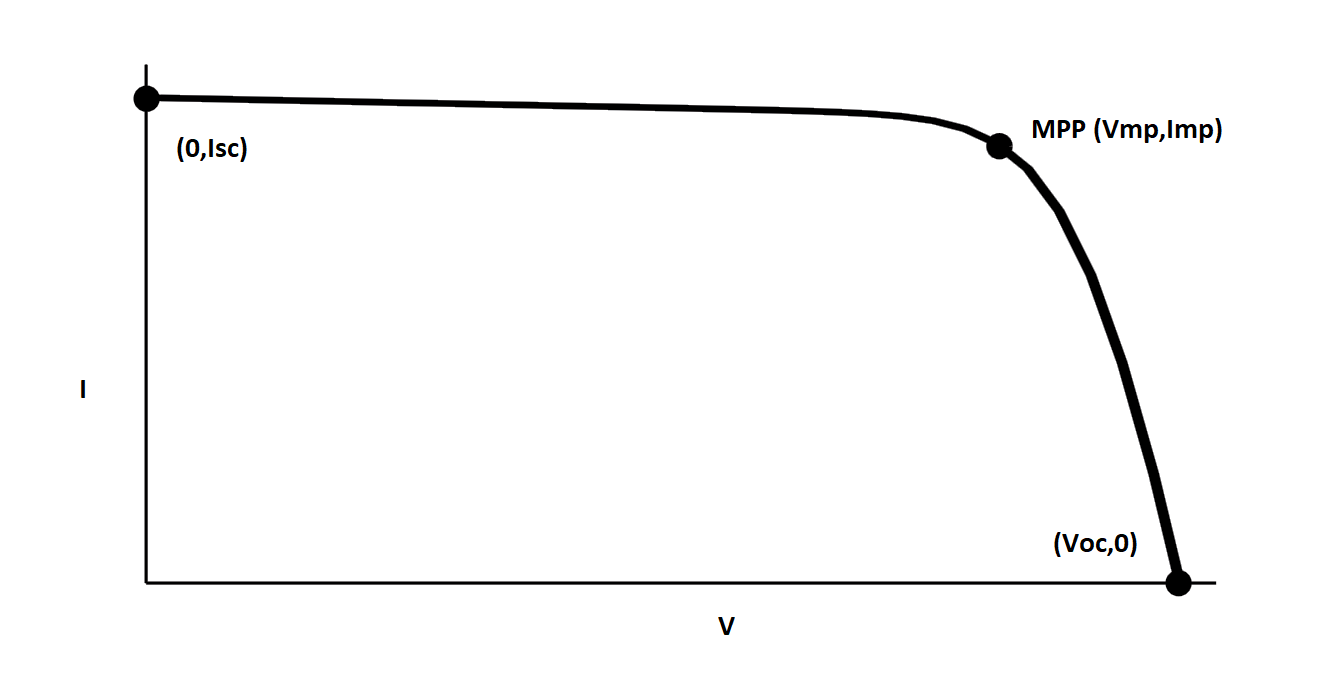
\includegraphics[width=10cm]{figuras/PV.png} 
\label{FigPVprofile}
\end{figure}
\par O modelo do painel solar fotovoltáico está na figura \ref{figPVsim}. Os resistores $R_p$ e $R_s$ podem ser estimados usando metódo interativo presente em \cite{VillalvaRuppert}. O resistor $R_p$ podem tem valor inicial dado por \ref{Rp} e $R_s \approx 0$.
\par Pela figura \ref{FigPVprofile}, nota-se que há um ponto de máxima potência (MPP). Para todos os outros pontos de tensão e corrente, a potência será menor que isso, acarretando perdas de eficiência do conjunto. 
\begin{equation}
    I=I_{pv}-I_o\big[ e^{(\frac{V+R_s.I}{V_t.a})} - 1 \big] - \frac{V+R_s.I}{R_p}
    \label{IPV}
\end{equation}
\begin{equation}
    V_t=\frac{N_s.k.T}{q}
    \label{IPV_Vt}
\end{equation}

\begin{equation}
    Rp_{min}=\frac{V_{mp}}{I_{sc}-I_{mp}} - \frac{V_{oc}-V_{mp}}{I_{mp}}
    \label{Rp}
\end{equation}
\begin{figure}[H]
\caption{Modelo do painel fotovoltáico. Retirada de \cite{VillalvaRuppert}} 
\begin{center}
\begin{circuitikz}
%Coluna,Linha
%(0,0) botton left
\draw
    (0,0)   to [short,-*] (6,0)
    (3.5,4) to [R, i=$I$, l_=$R_s$] (5.5,4)
    (5.5,4) to [short,-*] (6,4)
    (0,0)   to [american current source, l_=$I_{pv}$] (0,4)
    (0,4)   to [short] (3.5,4)
    (1.5,4) to [short, *-, i=$I_d$] (1.5,3) 
    (1.5,3) to [D] (1.5,1)
    (1.5,1) to [short,-*] (1.5,0) 
    (3,4)   to [R, *-*, l_=$R_p$] (3,0); 

\end{circuitikz}
\end{center}
\label{figPVsim}
\end{figure}




\section{Bateria de Íons de Litio}
\par Há vários métodos para carregamento de baterias de Íons de lítio.\cite{YONG2015365}. O método mais convencional e utilizado aqui será com corrente constante/tensão constante, representado na figura \ref{Figbatprofile}. Este método se utiliza de duas etapas: 
\begin{enumerate}
    \item CC - Mantém a corrente constante mesmo que a tensão caia abaixo do valor nominal de carregamento. 
    \item CV - Mantém a tensão constante até o fim do carregamento. 
\end{enumerate}

\begin{figure}[H]
\caption{Perfil de carga de bateria de Íons de litio. Retirada de \cite{YONG2015365}, traduzida pelo autor.}
 \centering % para centralizarmos a figura
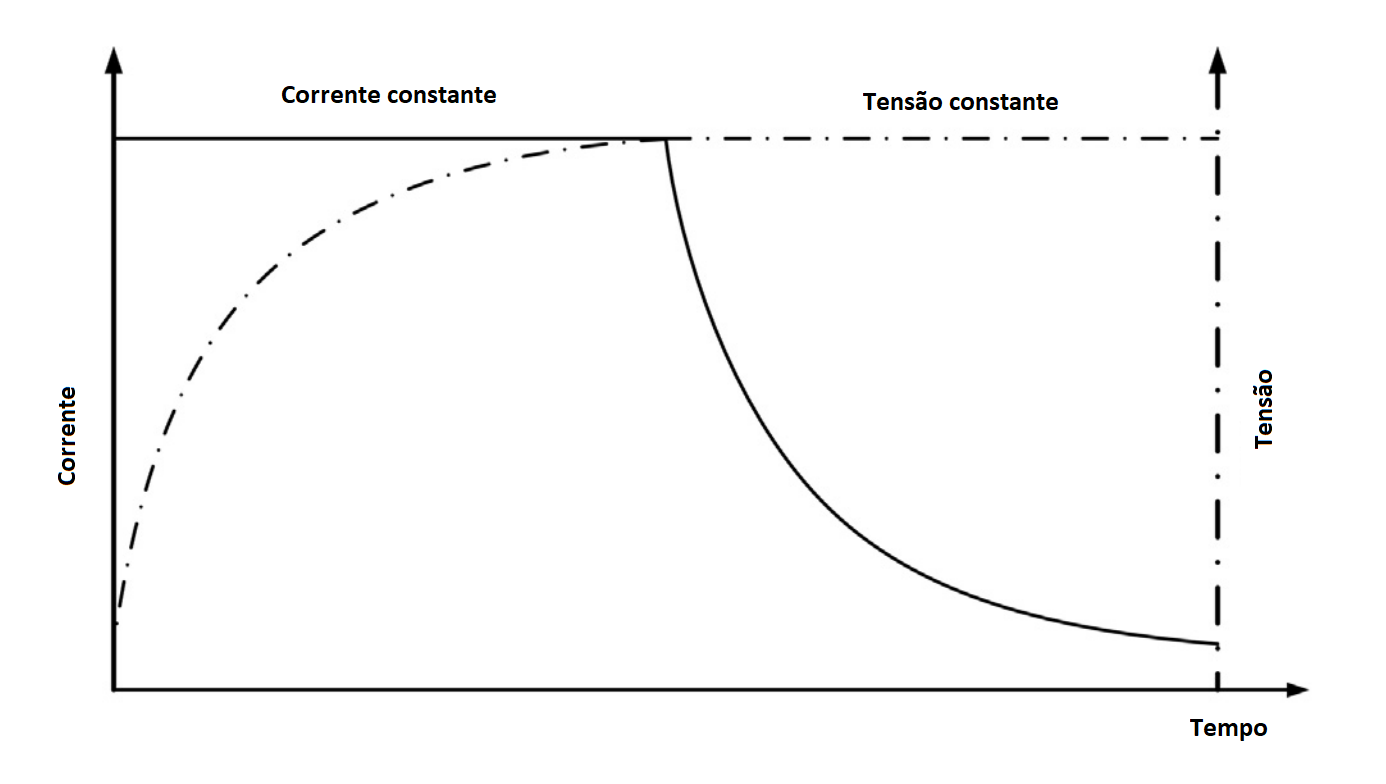
\includegraphics[width=10cm]{figuras/BateriaProfile.png} 
\label{Figbatprofile}
\end{figure}
